%----------------------------------------------------------------------------------------
% PACKAGES AND DOCUMENT CONFIGURATIONS
%----------------------------------------------------------------------------------------

  \documentclass[12pt]{article}

  \usepackage{hyperref}
  \usepackage{fancyhdr} % Required for custom headers
  \usepackage{lastpage} % Required to determine the last page for the footer
  \usepackage{extramarks} % Required for headers and footers
  \usepackage[usenames,dvipsnames]{color} % Required for custom colors
  \usepackage{graphicx} % Required to insert images
  \usepackage{listings} % Required for insertion of code
  \usepackage{courier} % Required for the courier font
  \usepackage{lipsum} % Used for inserting dummy 'Lorem ipsum' text into the template
  \usepackage{wrapfig}
  \usepackage{color}
  \usepackage{lscape}

  \setlength\parindent{0pt} % Removes all indentation from paragraphs
  \renewcommand{\labelenumi}{\alph{enumi}.} % Make numbering in the itemize environment by letter rather than number (e.g. section 6)

  % Margins
  \topmargin=-0.7in
  \evensidemargin=0.2in
  \oddsidemargin=-0.2in
  \textwidth=7.0in
  \textheight=9.0in
  % \headsep=0.25in

  % \linespread{1.1} % Line spacing

  \definecolor{dkgreen}{rgb}{0,0.6,0}
  \definecolor{gray}{rgb}{0.5,0.5,0.5}
  \definecolor{mauve}{rgb}{0.58,0,0.82}
  \definecolor{greyish}{rgb}{0.96,0.96,0.96}

  \lstset{
    backgroundcolor=\color{greyish},   % choose the background color; you must add \usepackage{color} or \usepackage{xcolor}
    frame=tblr,
    numbers=left,                       % where to put the line-numbers; possible values are (none, left, right)
    numbersep=5pt,                   % how far the line-numbers are from the code
    numberstyle=\tiny\color{mygray}, % the style that is used for the line-numbers
    language=Prolog,
    aboveskip=3mm,
    belowskip=3mm,
    showstringspaces=false,
    columns=flexible,
    basicstyle={\footnotesize\ttfamily},
    numbers=none,
    numberstyle=\tiny\color{gray},
    keywordstyle=\color{blue},
    commentstyle=\color{dkgreen},
    stringstyle=\color{mauve},
    breaklines=true,
    breakatwhitespace=true
    tabsize=3
  }

  \begin{document}
  \begin{titlepage}

%----------------------------------------------------------------------------------------
% TITLE PAGE INFORMATION
%----------------------------------------------------------------------------------------
 \newcommand{\HRule}{\rule{\linewidth}{0.5mm}} % Defines a new command for the horizontal lines, change thickness here
  \begin{center} % Center everything on the page

  %----------------------------------------------------------------------------------------
  % HEADING SECTIONS
  %----------------------------------------------------------------------------------------
  \textsc{\large Faculty of Computers, Informatics and Microelectronics}\\[0.5cm]
  \textsc{\large Technical University of Moldova}\\[1.2cm] % Name of your university/college
  \vspace{35 mm}
  \textsc{\Large PLIA}\\[0.5cm] % Major heading such as course name
  %\textsc{\large Laboratory work \#1-3}\\[0.5cm] % Minor heading such as course title
  \textsc{\large Laboratory work \# 1}\\[0.5cm] % Minor heading such as course title

  %----------------------------------------------------------------------------------------
  % TITLE SECTION
  %----------------------------------------------------------------------------------------
  \vspace{10 mm}
  \HRule \\[0.4cm]
  { \LARGE \bfseries Introduction of Programming Language Prolog}\\[0.4cm] % Title of your document
  \HRule \\[1.5cm]

  %----------------------------------------------------------------------------------------
  % AUTHOR SECTION
  %----------------------------------------------------------------------------------------
      \vspace{35mm}

      \begin{minipage}{0.4\textwidth}
      \begin{flushleft} \large
      \emph{Author:}\\
      Petru \textsc{Negrei} % Your name
      \end{flushleft}
      \end{minipage}
      ~
      \begin{minipage}{0.4\textwidth}
      \begin{flushright} \large
      \emph{Supervisor:} \\
      L. \textsc{Luchianov} % Supervisor's Name
      \end{flushright}
      \end{minipage}\\[4cm]

      \vspace{5 mm}
      % If you don't want a supervisor, uncomment the two lines below and remove the section above
      %\Large \emph{Author:}\\
      %John \textsc{Smith}\\[3cm] % Your name

      %----------------------------------------------------------------------------------------
      % DATE SECTION
      %----------------------------------------------------------------------------------------

      {\large Octomber 2014}\\[3cm] % Date, change the \today to a set date if you want to be precise

      %----------------------------------------------------------------------------------------
      % LOGO SECTION
      %----------------------------------------------------------------------------------------

      %\includegraphics{Logo}\\[1cm] % Include a department/university logo - this will require the graphicx package

      %----------------------------------------------------------------------------------------

      \vfill % Fill the rest of the page with whitespace
      \end{center}
      \end{titlepage}

      % \newpage
      % \tableofcontents
      % \newpage

%----------------------------------------------------------------------------------------
% Introduction
%----------------------------------------------------------------------------------------

  \section{Introduction}

  \subsection{Topic}

   Introduction of Programming Language Prolog

  \subsection{Objective}

  Main principles of working with programming language Prolog.

  \subsection{Generic requirements}

  \subsubsection{Task}

  \begin{itemize}
    \item Read the instructions and  necessary theory.
    \item Analyze given examples and find alternative solutions (questions).
    \item Elaborate your family tree and a knowlegde base in Prolog which will
    describe existing relations in your family and that will provide questions to them.
    Your family tree contain at least three generations. In order to check relations will
    be used at least six scopes.
  \end{itemize}

  \subsubsection{Report}

  Report will containt a short description of work done, and will present necessary information
  about tools, algorithms used or studied.

%----------------------------------------------------------------------------------------
% Implementation
%----------------------------------------------------------------------------------------

  \section{Implementation}

    \begin{itemize}
      \renewcommand{\labelitemi}{$\circ$}
      \item \textit{data}  (or ``raw'' data) is computer data without any concern for its meaning.
      \item \textit{Information} is data with a meaning, data that means something.
      \item A \textit{data base} is a collection of information that allows one to extract meaningful data in many different ways.
      \item A \textit{knowledge base} has even more: in addition to the information (called \textit{facts} in prolog), and the ability to extract information,
      there is also the ability to deduce new facts using prolog \textit{rules}.
    \end{itemize}

    \subsection{Facts}

    Here are some facts for a simple prolog knowledge base. It gives facts about a small family tree, with part of three generations.
    Below you can see a graphical representation of family tree.

    \newpage

    \begin{minipage}[b]{1.0\linewidth}
      \begin{center}
        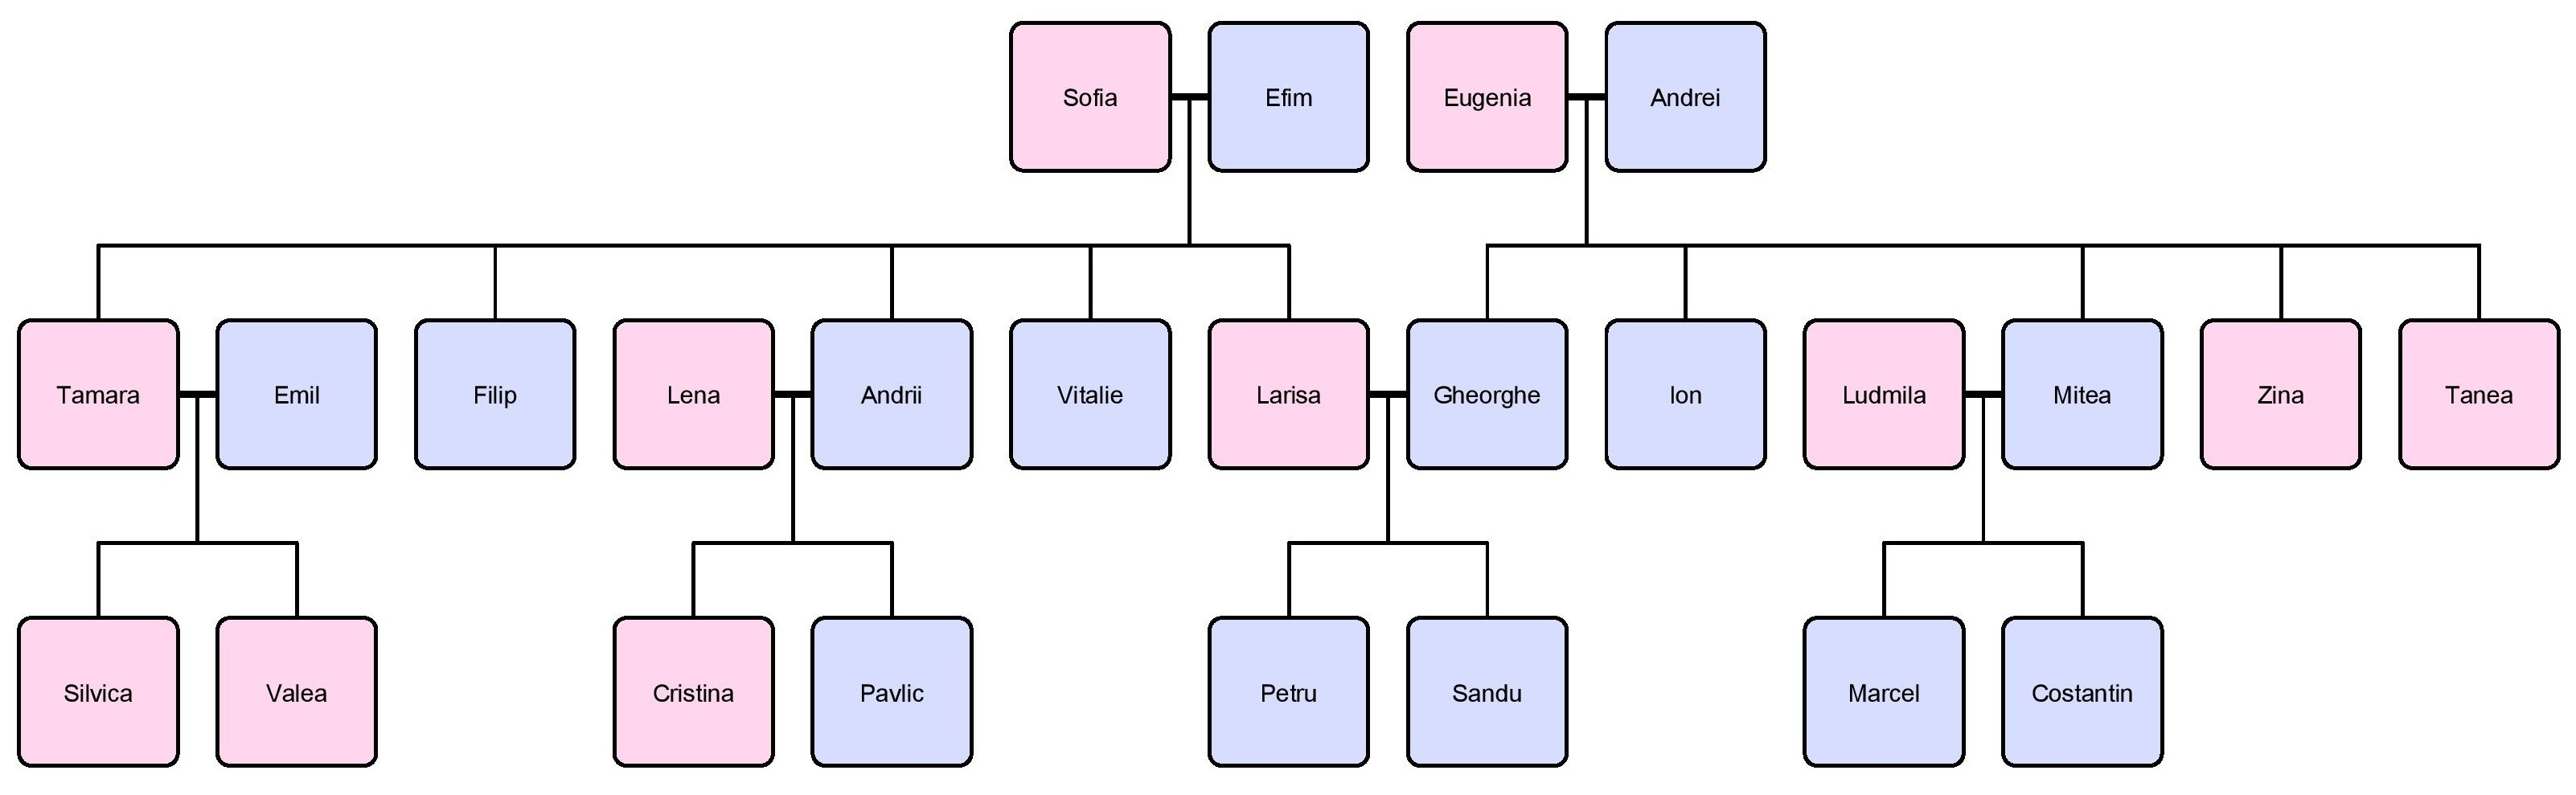
\includegraphics[width=1.0\textwidth]{plia3}
         \\ Fig. 1 Genealogical tree
      \end{center}
    \end{minipage}

    \vspace{0.5cm}

   Below is represented the full list of facts:

    \begin{lstlisting}
    male(petru).
    male(sandu).
    male(gheorghe).
    male(ion).
    male(mitea).
    male(andrei).
    male(vitalie).
    male(efim).
    male(andrii).
    male(filip).
    male(emil).
    male(pavlic).
    male(marcel).
    male(constantin).
    female(larisa).
    female(zina).
    female(tanea).
    female(eugenia).
    female(sofia).
    female(tamara).
    female(silvica).
    female(valea).
    female(cristina).
    female(lena).
    female(ludmila).
    parent(gheorghe, petru).
    parent(gheorghe, sandu).
    parent(larisa, petru).
    parent(larisa, sandu).
    parent(andrei, gheorghe).
    parent(andrei, ion).
    parent(andrei, mitea).
    parent(andrei, zina).
    parent(andrei, tanea).
    parent(eugenia, gheorghe).
    parent(eugenia, ion).
    parent(eugenia, mitea).
    parent(eugenia, zina).
    parent(eugenia, tanea).
    parent(efim, larisa).
    parent(efim, filip).
    parent(efim, andrii).
    parent(efim, tamara).
    parent(efim, vitalie).
    parent(sofia, larisa).
    parent(sofia, filip).
    parent(sofia, andrii).
    parent(sofia, tamara).
    parent(sofia, vitalie).
    parent(tamara, silvica).
    parent(tamara, valea).
    parent(emil, silvica).
    parent(emil, valea).
    parent(lena, cristina).
    parent(lena, pavlic).
    parent(adrii, cristina).
    parent(adrii, pavlic).
    parent(ludmila, marcel).
    parent(ludmila, constantin).
    parent(mitea, marcel).
    parent(mitea, constantin).
    married(andrei, eugenia).
    married(eugenia, andrei).
    married(efim, sofia).
    married(sofia, efim).
    married(gheorghe, larisa).
    married(larisa, gheorghe).
    married(emil, tamara).
    married(tamara, emil).
    married(lena, andrii).
    married(andrii, lena).
    married(ludmila, mitea).
    married(mitea, ludmila).
    \end{lstlisting}

    \subsection{Rules}

    \begin{lstlisting}
    husband(X, Y):-  male(X), married(X, Y).
    wife(X, Y) :-  female(X), married(X, Y).
    father(X, Y):-  male(X), parent(X, Y).
    mother(X, Y):-  female(X), parent(X, Y).

    sibling(X, Y) :-   father(Z, X), father(Z, Y),
                                mother(W, X),  mother(W, Y), not(X = Y).
    brother(X, Y) :-  male(X), sibling(X, Y).
    sister(X, Y):-  female(X), sibling(X, Y).

  \end{lstlisting}

  \newpage

  \begin{lstlisting}
    grandparent(X, Z):-  parent(X, Y), parent(Y, Z).
    grandfather(X, Z) :-  male(X),       grandparent(X, Z).
    grandmother(X, Z):-  female(X),     grandparent(X, Z).
    grandchild(X, Z) :-  grandparent(Z, X).
    grandson(X, Z) :-  male(X),  grandchild(X, Z).
    granddaughter(X, Z) :-  female(X),  grandchild(X, Z).

    child(Y, X) :-  parent(X, Y).
    son(Y, X) :-  male(Y),       child(Y, X).
    daughter(Y, X) :-  female(Y),     child(Y, X).

    auntoruncle(X, W) :-  sibling(X, Y), parent(Y, W).
    uncle(X, W) :-  male(X),       auntoruncle(X, W).
    aunt(X, W) :-  female(X),     auntoruncle(X, W).

    cousin(X, Y) :-  parent(Z, X),  auntoruncle(Z, Y).
    nieceornephew(X, Y) :-  parent(Z, X),  sibling(Z, Y).
    nephew(X, Y) :-  male(X),       nieceornephew(X, Y).
    niece(X, Y) :-  female(X),     nieceornephew(X, Y).
    \end{lstlisting}

    \section{Conclusion} % (fold)
    \label{sec:conclusion}

    In the following laboratory work I learn more about the fundamental part of
    the programming language Prolog. I build a knowledge base of my family tree using
    Prolog, writing facts and rules in order to provide necessary information based on external queries.


    % section conclusion (end)


\end{document}